\section{Theorie}

Myonen werden in der Atmosphäre durch Kollision von Teilchen dort mit Protonen aus extragalaktischen Quellen erzeugt. Da sie sich mit relativistischer Geschwindigkeit bewegen, erreichen sie trotz ihrer kurzen Lebensdauer den Erdboden. Der Zerfall in ein Elektron und zwei Neutrinos kann mit Hilfe eines geeigneten Versuchsaufbaus gemessen und so die Lebensdauer der Myonen bestimmt werden.

\subsection{Eigenschaften von Myonen}

Durch die Kollision von Protonen aus extragalaktischen Quellen wie z. B. Supernova-Überresten und aktiven Galaxienkernen werden Pionen erzeugt, welche in Myonen und Antimyonen zerfallen.
\begin{align}
	\pi^- \to \mu^- + \bar{\nu_\mu} \quad \text{bzw.} \quad \pi^+ \to \mu^+ + \nu_\mu
\end{align}
Mit einer durchschnittlichen Energie von $\SI{4}{\mega\electronvolt}$ \cite{PGD} sind Myonen relativistisch und können trotz einer Lebensdauer von $\SI{666}{\micro\second}$ \cite{PDG} den Erdboden erreichen.\par
Myonen sind Leptonen, besitzen einen Spin von $\hbar/2$ und gehorchen der Fermi-Dirac-Statistik. Sie gehören zur zweiten Leptonengeneration und haben eine Masse von $\SI{206}{\mega\electronvolt}$. Sie zerfallen in ein Elektron und zwei Neutrinos:
\begin{align}
	\mu^- \to e^- + \bar{\nu_e} + \nu_\mu \quad \text{bzw.} \quad \mu^+ \to e^+ + \nu_e + \bar{\nu_\mu}.
\end{align}
Das Myon kann auch anstelle eines Elektrons durch ein Atom gebunden werden, dieser Prozess ist allerdings sehr selten.

\subsection{Definition der Lebensdauer}

Die Wahrscheinlichkeit $\text{d}W$, dass ein instabiles Teilchen in einem infinitesimalen Zeitraum $\text{d}t$ zerfällt ist konstant $\lambda$, wobei diese Konstante spezifisch für eine Teilchensorte ist. Wenn eine Anzahl $N$ Teilchen vorhanden ist, ist die Änderung der Teilchenzahl $\text{d}N$
\begin{align}
	\text{d}N = -N\,\text{d}W = -N\lambda\,\text{d}t
\end{align}
lediglich von der Zerfallskonstanten $\lambda$ und der Zeitdauer abhängig. Integration liefert dann die Teilchenzahl zu einem beliebigen Zeitpunkt $t$
\begin{align}
	N(t) = N_0 \exp{-\lambda t}.
\end{align}
Wenn die Verteilung der Lebensdauer $t$ der Teilchen einer Exponentialverteilung
\begin{align}
	\frac{\text{d}N(t)}{N_0} = \lambda \exp{-\lambda t}\,\text{d}t
\end{align}
folgt, ist ihre charakteristische Lebensdauer $\tau = 1/\lambda$.

\begin{figure}[h]
	\centering
	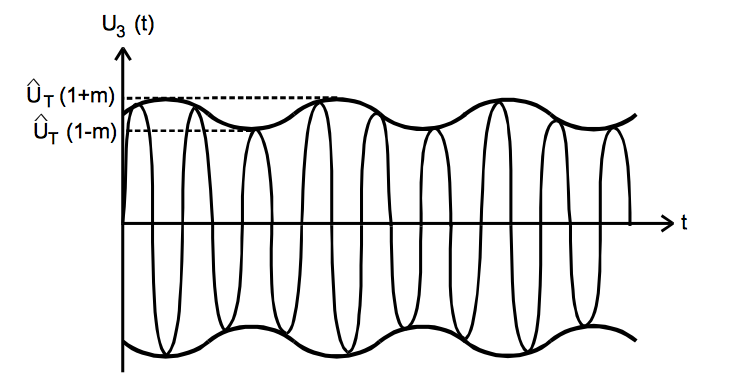
\includegraphics[width=\textwidth]{img/Abb1.png}
	\caption{Zeitabhängigkeit der Signalspannung eines Amplitudenmodulierten Signals \cite{FP}}
\end{figure}
